%Subphases
\chapter{Contextual Analysis}
Once the source code has passed through the syntax analysis, and thereby is validated in regard to the \acrshort{cfg}, it must be checked for contextual errors.\todo{Nu er der 2 gange rød tråd, skal vi slette det i det forhenværende eller er det fint at beholde begge? - Søren Det ser fint ud for mig -- MP - det virker fint som en indledning til afsnittet - Marc}

In the contextual analysis phase semantic errors are the ones being checked for\todo{En sætning som denne indeholder imo alt for mange fyldord, kunne have været: ``The contexual analysis checks for semantic errors'' -- Troels}, this includes type errors such as type mismatch, e.g. adding a boolean to a float, which may well be adhering to the grammar, but is not a valid arithmetic expression in \gls{gamble}.
Scope checking is also done in the contextual analysis. 
The design and implementation of the contextual analysis as well as how such errors are handled are described in this chapter.

The contextual analysis phase has sub-phases for scope- and type-checking and error reporting.
An illustration of the design for this can be seen on \myref{fig:flowContextual}, both sub-phases scope-checker and type-checker will have its own visitor class implemented.
The diagram shows that if variables are out of scope or type mismatches, it results in errors which will stop the compilation, if no errors occur it results in a decorated \acrshort{ast} which is then used in the next phase of the compiler, code generation.

%\begin{figure}[ht]
%  \centering
%    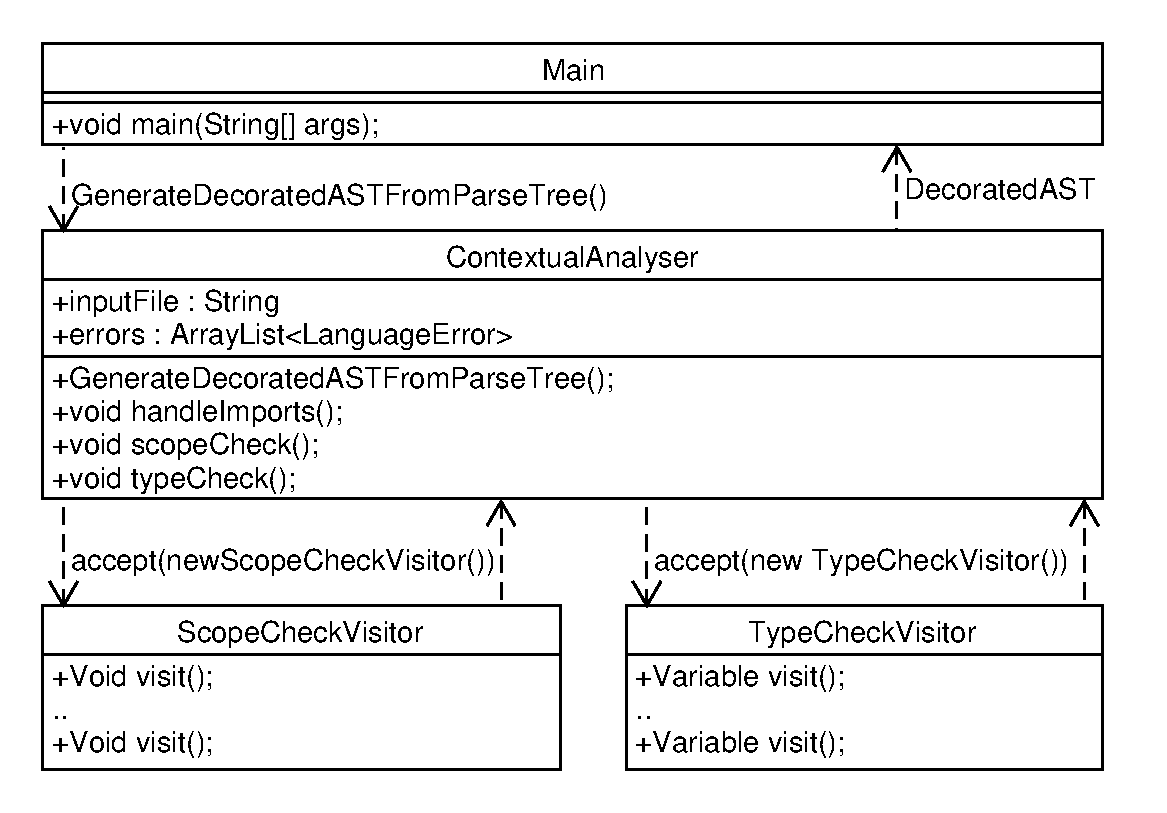
\includegraphics[width=0.48\textwidth]{figures/ClassDiagrams/ContextualAnalyser.pdf}
%  \caption{The function calls and returns in the Contextual Analysis phase.}
%  \label{fig:Contextual}
%\end{figure}

\vspace{10pt}
\begin{figure}[h]
    \centering
    \begin{tikzpicture}[node distance = 3cm, auto]
        \node (invi1) [invi, draw=none] {};
        \node (snyanal) [lille, below right=-2cm and -1.6cm of invi1, minimum width=15.5cm, minimum height=5cm, fill=blue!10, label={[xshift=-5.4cm, yshift=-1cm]Contextual Analysis}] {};
        \node (ast) [lille, below right=-0.35cm and -1cm of invi1] {Abstract Syntax Tree};
        \node (symboltable) [lille, minimum width=6.75cm, minimum height=2.4cm, right=2.8cm of invi1, fill=blue!20, label={[xshift=0cm, yshift=-1cm]Symbol Table}] {};
        \node (scope) [lille, right=1.1cm of ast] {Scopechecker};
        \node (type) [lille, right=0.7cm of scope] {Typechecker};
        \node (dast) [lille, right=1.1cm of type, align=left] {Decorated\\ Abstact Syntax Tree};
        \node (codegen) [lille, right=1.1cm of dast, align=left] {Code \\Generation};

        \node (error) [invi, draw=none, minimum width=2cm, below=1cm of symboltable, label={[xshift=40pt, yshift=-17pt]Error report}] {};

        %\node (error) [draw=none, above=22pt of parser, label={[xshift=0cm, yshift=6 pt]Error report}] {};

        \draw[black,fill=black, above=1cm of parser] (6.35,-2.5) circle (1ex);
        \draw[black, above=1cm of parser] (6.35,-2.5) circle (1.3ex); 

        \draw [arrow] (ast) -- (scope);
        \draw [arrow] (scope) -- (type);
        \draw [arrow] (type) -- (dast);
        \draw [arrow] (dast) -- (codegen);

        \draw [arrow,dashed] (scope) -- (error);
        \draw [arrow,dashed] (type) -- (error);
        \draw [arrow,dashed] (symboltable) -- (error);

    \end{tikzpicture}
    \caption{State diagram showing the modules of the contextual analysis. } 
    \label{fig:flowContextual}
\end{figure}
\vspace{-20pt}

%\section{Contextual Analysis}
\info[inline]{meta for this, phases are done in their own subsection files}
\section{Symbol Table}
In a compiler it is useful to store information about the identifiers, variables and functions in a data structure. 
This information can be useful for scope checking and type checking.

There are two common ways of implementing a Symbol Table; either you have one table which contains every identifier or you have a Symbol table for each scope. 
If constrained by memory, having a single symbol table can be beneficial, however having multiple symbol tables can simplify the code at a memory cost. 

In \gls{gamble} there exists scopes, and for each of these scopes there is a corresponding symbol table. 
Scopes inherit from each other so a scope can enclose another. 
The outermost scope, the global scope, is where functions are declared; every scope is either directly enclosed by this scope or recursively.
This means that every function can be called from anywhere within the source code - including within its' own function declarations; allowing for recursive functions. 
  

\info[inline]{Flyttes til implementationsafsnit $\downarrow$ }
In \gls{gamble} the class \texttt{SymbolTable} represents the symbol table.
The core constituent of this class is the ArrayList of the Scope class, called allScopes, meaning that every scope is stored in this ArrayList.
Every scope contains Map of Symbols and strings as keys, and information about the scope such what scope it is enclosed by. 
The key represents the name of the symbol, and must be unique to the scope and not found in an enclosing scope, as this could cause an ambiguity to arise. 
A symbol is either a variable or a function, in the class Symbol its data type, name and scope is stored. 


\section{Scope Checking}
As a part of the contextual analysis the compiler must ensure that every reference is valid in their given scope.
The validity of such reference is specific to the rules of the language, this section describes how the compiler upholds the rules listed in \myref{subsec:Scope}.
\subsection*{Design}
In \myref{subsec:Scope} the scope of identifiers, variables and functions, are defined for \gls{gamble}.
A variable is in scope from its declaration until the end of the block it is declared in.
An inner scope inherits the identifiers declared in the outer scopes. 

In the contextual analysis part of the compiler it is important to verify that each variable and function used are in scope, and it should produce a useful error message.
The error message should indicate which identifier is not in scope, and on what line this identifier is used wrongly.

To check this all references to identifiers must be checked to see if they match an identifier in the symbol table of the current scope, and recursively the scope which encloses it. 
Furthermore it is important that any usage of an identifier only exists after its declaration.
In the compiler for this project, the symbol table is filled while the compiler is also performing the scope checking.
This is because it reduces the amount of traversals through the tree, and scope checking and filling the symbol table is also similair in concept, e.g. a declaration creates an entry in the symbol table, while expressions simply make lookups in this table.

The scope checker produces two errors: redeclaration errors and undeclared errors.
A redeclaration error is produced when an attempt to declare a variable while it is already declarared in scope is made.
An undeclared error is produced when an attempt to use a variable which is not declared in the current scope or any enclosing scopes is made. 
Examples are shown in \myref{lst:scopeErrors}.

\begin{lstlisting}[caption=Examples of scope errors in \gls{gamble}, numbers=none,frame=tlrb,label={lst:scopeErrors}]
/* [...] */
int a = 1;
float a = 2.2;   /* Redeclaration error */
int a = 2;       /* Redeclaration error */ 

b = 2;           /* Undeclared error */   
int b = 0;
b = foo();       /* Redeclaration error and undeclared error */ 
/* [...] */
\end{lstlisting}

\subsection*{Implementation}
In the \gls{gamble} compiler, the class \texttt{SymbolTable} represents a collection of scopes.
The core constituent of this class is the ArrayList of the \texttt{Scope} class, called \texttt{allScopes}, meaning that every scope is stored in this ArrayList.
Every scope contains a hashed map with \texttt{Symbol}s as values and strings as keys.
Furthermore all scopes contain information about the particular scope such as enclosing scope and a unique id. 
The key in the hashed maps represents the name of the symbol, and must be unique to the scope and not found in an enclosing scope, as this could cause an ambiguity to arise.
This ambiguity is not allowed in \gls{gamble} and therefore generates a redeclaration error.
To determine wether or not a declaration is a redeclaration, the compiler looks up the name of the variable in the \texttt{symbolMap} of the current scope.
If no entry is found, the search continues in the \texttt{symbolMap} of the enclosing scope and outwards.
The same lookup process is executed when a variable is used e.g in a expression or assignment.
Hereby all enclosing scopes are checked for the declaration of the variable; making redeclaration of variables in scope, and usage of undeclared variables impossible in \gls{gamble}.
A symbol is an encapsulation of a variable and relevant peripheral data.
The peripheral data consists of a boolean, used for checking is a declared variable is used, and an integer with the line number if the declaration of the variable.
The boolean describing if a declared variable is used, is set to true, if the previously described lookup process for a variable in use, finds a declared variable from the unique id (the name if the variable).
This boolean also makes it possible for the \gls{gamble} compiler to find unused variables and then prompt the user with a relevant warning.

In order for all of the above to be implemented an instance of the \texttt{SymbolTable} class is passed via the constructor, to a visitor which traverses the \acrfull{ast}.
This visitor, the \texttt{SymbolTableFillVisitor} then fill the referenced \texttt{symbolTable} with scopes and their symbols.
Every time the visitor meets the start of a new scope e.g. the block of statements within a loop construct.
A new instance of the \texttt{Scope} class is pushed to the \texttt{scopeStack}, hereby making it possible to fill the relevant scope when the block of statements is visited.
At the end of a scope the top element on the \texttt{scopeStack} is popped off, and as a consequence of this the top of the \texttt{scopeStack} is back to the enclosing scope.

\section{Type Checking}
Another important part of the contextual analysis phase for the compiler is the type checking, which enforces the type system of \gls{gamble}.
This section will cover the design and implementation of the type checking in the compiler.
\subsection*{Design}
The second important part of the contextual analysis phase for the compiler is the type checking, which enforces the type system of \gls{gamble}.
As \gls{gamble} is statically typed it is necessary to check if all references to identifiers and constant values fit into the context they exist in. 
Since implicit conversion between floating point and integer types is not a part of \gls{gamble} an error must be issued everywhere they are used wrongly. 
It is however possible to implicitly convert between integer and floating point types internally e.g. from int16 to int64, as long as the destination variable is of a larger bit-width.
This is also the case for complex datatypes, matrices and vectors, e.g. from \texttt{matrix<float>} to \texttt{matrix<float64>}. 

The symbol table is used as a reference for which type the variable is, and therefore the type checking happens after the symbol table has been filled, hence after scope checking is completed. 
Type checking is done in many parts of the code, one or more times for each line is common. 
For every operator it must be checked if its types match and if it results in an assignment if that also matches.
Every function call must match the formal parameters of the function. 

The errors produced by the type checker are: Argument errors and type mismatch errors.
An argument error indicates that the number of arguments in the function declaration does not match the number of arguments provided in the function call.
A type mismatch error is caused by a value or identifier not being compatible (type safe) with the function parameters, operator used etc.
Examples are shown in \myref{lst:typeErrors}.

\begin{lstlisting}[caption=Examples of type errors in \gls{gamble},numbers=none,frame=tlrb,label={lst:typeErrors}]
/* [...] */
int a = 1 + 2;      /* Valid */
float b = 2.2 + 1;  /* Type mismatch error */
float c = 2;        /* Type mismatch error */

a = 2.2;            /* Type mismatch error */
b = foo(1);         /* Argument error (Takes more or fewer arguments) */ 
/* [...] */
\end{lstlisting}

\subsection*{Implementation}
The type checker is called right after the symbol table has been filled by the \texttt{SymbolTableFillVisitor}.
Since \gls{gamble} is static typed, the type checker is implemented under the contextual analysis phase of the compiler, in contrast to a dynamically typed language, such as Python or R, which is checked at runtime. \todo{er dette nødvendigt. MP}
\gls{gamble} validates the size of matrices and vectors match for certain operations as addition and multiplication E.g., as well as if they are out of bounds. 
This is to make it easier for the programmers using \gls{gamble} at a cost of speed. 
To implement type checking in the \gls{gamble} compiler a visitor is used during the contextual analysis.
The class \texttt{ASTTypeCheckVisitor} visit every relevant node in the \acrshort{ast} to check for type errors.
The class collects a list of every type error it finds, these errors is then presented to the user, when a compilation fails.
Errors and error handling are further described in \myref{subsec:DesignErrorHandling}.
The class \texttt{ASTTypeCheckVisitor} overrides the visitor calls from the \texttt{baseASTVisitor} class.
The visitor does this in multiple places in the \acrshort{ast} and the visitor uses a class \texttt{TypeChecker}, which through method calls on the variables in the nodes.
\texttt{TypeChecker} contains a method, \texttt{CombineValueTypes} which takes two values and checks if they are type compatible.
\texttt{ASTTypeCheckVisitor} visits nodes which contains either one or more variables meaning that there can be errors which should be found. 
An example of this is seen in \myref{lst:typecheck1} where the method \texttt{VisitExpressionNode}
 is shown.
The method visits an \texttt{ExpressionNode} and calls \texttt{CombineValueTypes} with the nodes left and right values if there are any available else it send \texttt{null} as the input value.
The method visits an \texttt{ExpressionNode} and uses the the \texttt{TypeChecker}s \texttt{CombineValueTypes} method, the method checks the types of the children of the \texttt{ExpressionNode} and if they fits the operator then it returns the type of the expression. 
The method returns a variable of the type returned \texttt{ValueType} and string which is printed if the visit finds type errors.

\begin{lstlisting}[caption=The VisitExprressionNode method in the ASTTypeChecker class,numbers=none,frame=tlrb,label={lst:typecheck1}]
public Variable VisitExpressionNode(ExpressionNode node) {
    ValueType valueType = TypeChecker.CombineValueTypes(
            node.getLValue() != null ? visit(node.getLValue()) : null,
            node.getRValue() != null ? visit(node.getRValue()) : null,
            errors,
            node.getLineNumber()
    );
    node.setValueType(valueType);

    return new Variable(valueType, "Expr:<" + node.toString() + ">");
}
\end{lstlisting}

After the type checker have checked every expression in the source code, the compiler scans for unused variables and thereafter prints all these as warnings. 

\section{Error Handling}
Error handling is a descriptive section of how the compiler handles errors, and how error handling is implemented.
Error handling is referred to as detection and solving of programming errors.
Both errors at compile time and run time will be handled.
\subsection*{Design}\label{subsec:DesignErrorHandling}
The source code given to the \gls{gamble} compiler may contain errors and warnings, these errors are found and uncovered in various stages of the compiler.   
In the syntax analysis, all syntactic errors are found, and the compilation is stopped if errors are found, since it would not be advised to further compile source code, which contains fundamental syntactic errors.
However it should be noted that the entire syntax analysis is completed before stopping the compiler, hence all syntactic errors are collected and reported to the user.\todo{Et andet sted står der at hvis en fejl mødes bliver det abrupted det skal lige rettes så det passer med det her tror jeg :)(det er vist mig der skrev det bliver stoppet, jeg huskede forkert, I R SOWIE) - Søren}
This makes the process of resolving syntactic errors less tedious for the programmer, than if the compiler would stop every time a single error was detected. 
A core element of error handling is scope and type related errors, these are found in the previously explained subphases of the contextual analysis: Scope- and typechecking.
As with the syntactic analysis, the compiler collects all errors before stopping the compilation of the source code. 
The following errors and warnings are reported by the \gls{gamble} compiler:
\begin{description}
	\item[Argument error]\hfill\\ 
	The arguments required in a function call doesn't match the ones used.
	\item[Redeclaration error]\hfill\\ 
	A variable or function with the same name is already declared.
	\item[Type mismatch error]\hfill\\ 
	The type or types used are incompatible with each other and/or the operator. 
	\item[Undeclared error]\hfill\\ 
	Attempted use of an undefined variable or function.
	\item[Unused variable warning]\hfill\\ 
	A warning signalling that a variable or function is declared but never used.
\end{description} 
The errors in the compiler should give useful information about: Where the error is located in the source code and what variable(s) or function(s) was wrongly used.
This includes line numbers which then have to be carried over from the parse tree to the \acrshort{ast}.

\subsection*{Implementation}\label{subsec:ImplementationErrorHandling}
In the \gls{gamble} compiler the error handling is implemented by having a class \texttt{LanguageError} of which each specific error type inherits from.
The \texttt{LanguageError} superclass has information about the type of the error, an enumeration which is either \texttt{Error} or \texttt{Warning}. 
This is so because a program which has warning but no errors, should still compile, however any program with errors should not. 
Compared to printing any error when it was discovered and stopping compilation, this model allows the compiler to go through the entire \acrshort{ast} and discover every error as described above. 
It also unifies how errors are printed and shown to the user.
There is also an integer indicating which line the error is contained on.
This enhances the error reporting process, making it easier for users to debug. 
As an example the class for \texttt{UnDeclaredError} is shown in \myref{lst:undeclarederrorclass}.
Firstly there are variables which contain information needed to report the error to the programmer. 
Then there is a constructor which simply assigns all values given to it to the new object's fields.
Lastly there is the \texttt{toString} method which is overridden from the implementation in the \texttt{LanguageError} class. 
An example of an \texttt{UnDeclaredError} is: \texttt{Error[line   42]-> Undeclared variable towel in scope Local}, if the variable's ID was \texttt{towel}. %Sneaky H2G2 reference 

\begin{lstlisting}[caption=The UnDeclaredError class in the \gls{gamble} compiler,numbers=none,frame=tlrb,label={lst:undeclarederrorclass}]
public class UnDeclaredError extends LanguageError {
    private Variable unDeclaredVariable;
    private Scope scope;

    public UnDeclaredError(Variable unDeclaredVariable, Scope scope, int lineNum) {
        this.unDeclaredVariable = unDeclaredVariable;
        this.scope = scope;
        this.lineNum = lineNum;
        this.errorType = ErrorType.ERROR;
    }

    @Override
    public String toString() {
        String type = unDeclaredVariable.isFunction() ? "function " : "variable ";
        return super.toString() + String.format("Undeclared %6$s %1$s%4$s%3$s in scope %2$s%5$s%3$s",
                ANSI_RED, ANSI_BLUE, ANSI_RESET,
                unDeclaredVariable, scope, type);
    }
}
\end{lstlisting}

This error is found in the \texttt{CheckIfUndeclared} method in the \texttt{SymbolTableFillVisitor} shown in \myref{lst:CheckIfUndeclared}.
The method is called whenever a variable or function is invoked.
If the variable or function invoked is not declared, an error is added to a global list of errors. 
\begin{lstlisting}[caption=The CheckIfUndeclared method in the SymbolTableFillVisitor class in the \gls{gamble} compiler,numbers=none,frame=tlrb,label={lst:CheckIfUndeclared}]
public Void CheckIfUndeclared(Variable variable, StatementNode node) {
    Symbol tmpSymbol = symbolTable.currentScope().resolve(variable.getId());
    if (tmpSymbol != null) {
        /* Sets appropriate information to the 'variable' variable */
    } else {
        errors.add(new UnDeclaredError(variable, symbolTable.currentScope(), node.getLineNumber()));
        symbolTable.currentScope().define(variable);
    }

    return null;
}
\end{lstlisting}\todo{Stemmer det overens med den nye struktur der blev lavet hvor der kaldes en error class i main ?? - Søren}
